%%% mode: latex
%%% TeX-master: t
%%% End:

\chapter{绪论}
\label{cha:intro}

\section{研究背景与意义}\label{sec:general intro}
推荐系统\cite{rs}是互联网信息时代解决信息过载问题的重要工具。其通过分析用户行为数据和历史行为信息,提供相关性、多样性和新颖性的内容选择,帮助用户快速准确地找到感兴趣的信息、辅助用户做出更明智的决策。在互联网飞速发展的信息时代,推荐系统在电商、社交媒体、新闻阅读等领域发挥着重要的作用,逐渐成为学术界和工业界的研究热点\cite{Steffen:2009:UAI,Ai:2018:SIGIR,Ding:2020:NIPS}。

%推荐系统广泛使用了自监督学习的技术。受限于推荐系统的场景特征,获取准确的用户偏好标签用于训练推荐模型是昂贵的。目前许多最先进的推荐模型都借助于自监督学习(Self-supervised Learning, SSL)\cite{Liu:2021:TKDE}的技术,通过对输入数据进行某种变换或处理来提取自监督信号。常见的自监督信号例如“用户对已交互的物品偏好大于未交互物品”\cite{Steffen:2009:UAI,Jingtao:2019:IJCAI,Xiangnan:2020:SIGIR,Wang:2019:SIGIR},“用户物品二分图轻微扰动的语义不变性”\cite{shuai2022review,lightgcl:2023:ICLR,wu:2023:TKDE}等。这种使用自监督信号的训练的推荐模型也被称为自监督推荐\cite{SSR:2023:TKDE}(Self-supervised Recommendation, SSR),是自监督学习的一个重要应用领域。自监督推荐分利用输入数据中的内在关系设计自监督任务训练推荐模型,不仅可以减少对手动标注数据集的依赖,而且也有助于缓解传统推荐系统中的数据稀疏、虚假相关性和对抗性攻击等问题\cite{SSR:2023:TKDE,Liu:2021:TKDE}。

推荐系统广泛使用了自监督学习的技术\cite{SSR:2023:TKDE,Xiangnan:2020:SIGIR,Wang:2019:SIGIR,shuai2022review,guo2022miss,tao2022self,yao2021self,xia2021self,liu2021contrastive,yuan2021improving,wu2020ptum,ma2020disentangled,10.1145/3459637.3482426,10.1145/3404835.3462862,self:aug}。受限于推荐系统的场景特征,获取准确的用户偏好评分标签是昂贵的。目前许多最先进的推荐模型都借助自监督学习(Self-supervised Learning, SSL)\cite{tong2023emp,Liu:2021:TKDE,Chen:2020:NIPS,BYOL:2020:NIPS,wu:2023:TKDE,gsl:2023:TKDE}技术,设计自监督任务(预)训练模型编码用户物品特征表示,以预测个性化排序(下游任务)。例如,生成型(Generative)自监督任务训练推荐模型对输入数据进行重建\cite{sun2019bert4rec,geng2022recommendation,zhang:sigir};对比型(Contrastive)自监督任务训练推荐模型编码正负样本差异特征\cite{Steffen:2009:UAI,Jingtao:2019:IJCAI,Xiangnan:2020:SIGIR,Wang:2019:SIGIR,shuai2022review,lightgcl:2023:ICLR,wu:2023:TKDE}。这种基于自监督任务引导训练的推荐模型也被称为自监督推荐\cite{SSR:2023:TKDE}(Self-supervised Recommendation, SSR),是自监督学习的一个重要应用领域。自监督推荐充分利用输入数据中的内在关系提取自监督信号,不仅可以减少对手动标注数据集的依赖,而且也有助于缓解传统推荐系统中的数据稀疏、虚假相关性和对抗性攻击等问题\cite{SSR:2023:TKDE,Liu:2021:TKDE}。

基于对比学习(Constrastive Learning, CL)\cite{zhang:cl}的推荐算法是自监督推荐的主要实现形式\cite{SSR:2023:TKDE},也称为对比型推荐算法。推荐系统中常见的对比方式包括“已交互的物品偏好大于未交互物品”的偏好对比\cite{Steffen:2009:UAI,Jingtao:2019:IJCAI,Xiangnan:2020:SIGIR,Wang:2019:SIGIR},“图轻微扰动语义不变性”的图对比\cite{shuai2022review,lightgcl:2023:ICLR,wu:2023:TKDE}等。对比学习在计算机视觉、自然语言处理和信息检索领域取得了巨大的成功\cite{Oord:2018:arxiv,Chen:2020:ICML,BYOL:2020:NIPS,Khosla:2020:NIPS,graph:CL,graph:self,cl:bei,xiao:cl},在推荐任务中也有诸多优势,主要体现在:(1) 互信息优化:通过
优化对比损失,拉近锚点与正例的距离、推远锚点与负例的距离,实现对互信息的优化\cite{Oord:2018:arxiv,yang2021enhanced,cao2021bipartite,zhou2020s3}。(2) 避免过拟合:对比损失激励编码器编码不同样本的差异特征,免于对样本进行像素级信息重构,从而避免了模型的过拟合\cite{Oord:2018:arxiv}。(3) 排序导向:在偏好对比任务中,优化成对损失或对比损失,导致了对排序列表排序指标AUC和NDCG的优化\cite{Steffen:2009:UAI,Jiancan:2022:arxiv}。

%
%对比学习\cite{zhang:cl}是自监督推荐的主要实现形式\cite{SSR:2023:TKDE}。对比学习在计算机视觉、自然语言处理和信息检索领域取得了巨大的成功\cite{Oord:2018:arxiv,Chen:2020:ICML,BYOL:2020:NIPS,Khosla:2020:NIPS}。对比学习在推荐任务中也有诸多优势,主要体现在:(1) 互信息优化:通过
%优化对比损失,拉近锚点与正例的距离、推远锚点与负例的距离,实现对互信息的优化\cite{Oord:2018:arxiv,yang2021enhanced,cao2021bipartite,zhou2020s3}。(2) 避免过拟合:对比损失激励编码器编码不同样本的差异特征,免于对样本进行像素级信息重构,从而避免了模型的过拟合\cite{Oord:2018:arxiv}。(3) 排序导向:在“用户对已交互物品的偏好大于为交互物品”这个的对比任务中,优化成对损失或对比损失,导致了对排序列表排序指标AUC和NDCG的优化\cite{Steffen:2009:UAI,Jiancan:2022:arxiv}。


基于对比学习的推荐算法显著推动了自监督推荐的前沿\cite{SSR:2023:TKDE},受到了广泛的关注\cite{liu2021contrastive,10.1145/3477495.3532009,qiu2022contrastive,yu2023xsimgcl}。尽管该类方法在自监督设置下表现出了出色的泛化能力,\textbf{但与有监督设置下的对比型推荐算法存在较大差距}\cite{Chuang:2020:NIPS,SSR:2023:TKDE,Khosla:2020:NIPS,zhang:cl}:用于偏好对比的正负样本标签是“伪标签”\footnote{自监督学习和无监督学习的共性是都不涉及人工标注的标签\cite{He:2020:CVPR};区分在于,自监督学习通过从共现输入中导出“伪标签”来关联信息\cite{Liu:2021:TKDE}。},不同于“喜欢与否”的真实偏好标签。二者的不一致性,对学习准确的用户物品特征表示产生不利影响。如何从不完全标注的隐式反馈数据中学到良好的对比表示(Contrastive Representations),是自监督学习和对比学习的理论需要,也是提升个性化推荐系统准确性的现实需求。

\section{国内外研究现状}
\label{sec:requirement}
现实世界中,对样本的度量方式主要有两种,一是对样本进行逐个(Pointwise) 度量,例如测量电容的大小。在高自由度场景中,由于:(1)单个样本的绝对值度量不容易获取;(2)体现相互关系的度量只能以成对方式体现;(3)特定场景中更关注相对值的大小而非绝对值的大小,导致了成对(Pairwise)度量的出现。成对度量广泛存在于描述客观世界的数据中,度量的方式主要有:(1)成对比较,例如方案$i$比方案$j$好,体现的是强弱关系;(2)成对关系,例如网页$i$的超链接指向网页$j$,体现了相互依存和作用的关系。成对度量提供了从相互关系描述、分析、挖掘事物的视角,相比于逐个度量的方式,突出了数据内部的结构信息,能够更好地描摹客观世界的真实形态。

\vspace{-0.0011cm}
推荐系统通常收集到的数据是隐式反馈数据,如点击、购买、浏览等行为数据。贝叶斯个性化排序 (Bayesian Personalized Ranking, BPR)\cite{Steffen:2009:UAI}率先将隐式反馈数据转化为成对比较。具体而言,对于某个用户(锚点),已交互物品$i$被标记为正例,未交互的物品$j$被标记为负例,相应的正负例构成一个成对比较实例。基于“用户对正例偏好大于负例的偏好”的假设(自监督信号),BPR使用Bradley-Terry模型\cite{Bradley:1952:Biometrika,Luce:2005:JASA}建模成对比较的似然,并通成对比较的极大似然估计学习潜在的用户表示和物品表示,在推荐中被称为成对学习\cite{Steffen:2009:UAI,Steffen:2014:WSDM,Xiangnan:2020:SIGIR,Wang:2019:SIGIR}。这种由偏好对比引导的模型(预)训练任务,激励推荐模型给正例评分大于负例,从而导致了排序列表的AUC指标的优化\footnote{如不考虑正则化项,成对损失函数BPR与AUC指标定义相同,不同之处在于BPR把AUC指标中不可微的$0-1$损失$\ell_{0-1}(\cdot)$替换成了可微的替代损失$\log\sigma(\cdot)$\cite{Steffen:2009:UAI}。}。由于BPR设计的偏好对比与下游排序预测任务具有一致性,逐渐主导了从隐式反馈数据中学习排序的任务\cite{Weike:2013:IJCAI,Yu:2018:CIKM,Xiaoye:2011:MathProg,Xuejiao:2020:ASC,Qiu:2018:IS,Zhao:2019:FGCS}。

\vspace{-0.0011cm}
成对学习BPR根植于对比学习范式\cite{Xu:2022:arxiv}。特别是,BPR损失与噪声对比估计\cite{Gutmann:2010:ICAIS,gutmann:2012:JMLR}(Noisy Contrastive Estimation, NCE)损失具有完全等价的函数形式\cite{Liu:2021:TKDE},它们都是广泛使用的对比损失InfoNCE\cite{Oord:2018:arxiv}在负例个数设置为1时的特例。尽管它们的解释不同,BPR将优化目标解释为用户偏好正例强于负例的后验,InfoNCE将优化目标解释为从负例中区分出正例的后验,但实际上都描述了由模型参数化的正例得分大于负例得分的程度。随后,InfoNCE损失也广泛应用于推荐中的排序预测任务\cite{Jiancan:2022:arxiv,lightgcl:2023:ICLR}。文献\cite{Jiancan:2022:arxiv}进一步讨论了优化InfoNCE损失导致优化排序指标NDCG。

\vspace{-0.0011cm}
对比学习采用从比较中学习(learn-to-compare)\cite{Gutmann:2010:ICAIS}的范式,通过区分观察数据和噪声数据来使模型免于重建数据的像素级信息~\cite{Oord:2018:arxiv}。虽然表示编码器和相似性度量会因任务而异~\cite{Devlin:2018:bert,He:2020:CVPR,Dosovitskiy:2014:NIPS,Xiangnan:2020:SIGIR,Wang:2019:SIGIR,Wenqi:2021:KDD},但它们都共享将正样本和负样本进行对比的基本思想,通过优化对比损失~\cite{Wang:2020:ICML}来训练编码器,如NCE损失~\cite{Gutmann:2010:ICAIS},InfoNCE损失~\cite{Oord:2018:arxiv},Infomax损失~\cite{Hjelm:2018:Arxiv},渐进对比损失~\cite{Wang:2020:ICML}等。这些损失函数隐式~\cite{Oord:2018:arxiv}或显式~\cite{Hjelm:2018:Arxiv}地优化了已知数据和待预测数据互信息的下界。Arora等人~\cite{Saunshi:2019:ICML}为对比学习的泛化界限提供了理论分析。对比学习在不同领域的许多应用中都取得了显著成功~\cite{Henaff:2020:ICML,Khosla:2020:NIPS,Liu:2021:TKDE,Bachman:2019:NIPS,chen2020improved,Huang:2019:ICML,Wu:2018:CVPR,Zhuang:2019:CVPR}。除了互信息优化、防止模型过拟合等优势之外,对比学习在推荐任务中的突出优势体现在推荐任务和对比学习任务的一致性\footnote{这里的一致性是指,由成对损失和对比损失引导的预训练任务((Pretext Task)与下游排序预测任务是一致的,体现在预训练阶段的对比损失和下游任务的性能度量存在关联。}:优化对比损失导致排序列表排序指标的优化\cite{Steffen:2009:UAI,Jiancan:2022:arxiv}。

\vspace{-0.0011cm}
从对比学习的视角,后续的研究按照对比学习的关键组件可以归纳为,正例增强方法,负例采样方法,对比损失函数设计等工作。正例增强主要通过附属信息获取不同偏好强度的正例\cite{Qiu:2018:IS,Lerche:2014:RS,Wenhui:2019:WWW,Yu:2018:CIKM,Bin:2020:IS}构造更细粒度的偏好比较,以学习更准确的决策边界。由于附属信息有限,后续的工作设计了基于图增强的图对比任务提升学到的表示\cite{lightgcl:2023:ICLR,ren2023disentangled,he2023candidate,yang2023generative};
%通过对比原图和增强图,学习体现用户物品二分图中重要的结构信息的节点特征表示\cite{lightgcl:2023:ICLR,ren2023disentangled,he2023candidate,yang2023generative};
负例的采样方法围绕采样困难负样本\cite{Steffen:2014:WSDM,Zhang:2013:SIGIR,Zhao:2015:CIKM,shi2023theories},且避免采样伪负样本\cite{Ding:2020:NIPS,Qin:2021:AAAI,Zhao:2021:IJCAI,Chen:2017:KDD,Mikolov:2013:NIPS,Weike:2013:IJCAI,Yu:2018:CIKM,Wang:2019:SIGIR}这两个目标展开,以激励模型更准确地学习兴趣边界。在损失函数设计上,主要是将排序导向的偏好对比任务和图对比任务组合,将原始的单一对比目标向多个对比目标进行拓展,使得最终的优化目标同时约束排序目标和保留用户物品二分图结构信息的目标\cite{Wang:2022:KDD,ren2023disentangled,lightgcl:2023:ICLR,he2023candidate,zhu2023adamcl,qin2023meta,shuai2022review}。


\section{关键问题}
在推荐系统中,正例的语义为“喜欢的物品”,负例的语义为“不喜欢的物品”。然而,用户通常只通过交互行为(如点击、购买)来表达偏好或兴趣。一方面,这些交互行为通常不包含显式的评分,只能观测到交互的有无,无法观测到交互数据所对应的偏好强度高低。不体现偏好的交互如代购、误触、查看等异常模式与正常交互无法区分,都被标记为正例\cite{Yu:2018:CIKM,Qiu:2018:IS,Wang:2021:WSDM}。另一方面,由于用户仅仅提供正反馈,无法观测到用户不喜欢哪些物品,所有用户未看见的物品都被标记为负例,但它们实际上是未标注数据\cite{Ding:2020:NIPS,Zhang:2013:SIGIR,Yang:2020:KDD}。因此,用于训练推荐系统的数据集通常以正例-未标注(Positive-Unlabeled, PU)形式存在,且正例还含有噪声。依照隐式反馈数据交互的有无获取的正负样本的“伪标签”,与真实的偏好标签具有不一致性。这一现象,导致自监督设置下的对比型推荐算法存在以下问题:
\begin{enumerate}
\item \textbf{伪正例问题}

~~~~~~~~正例(已交互物品)不代表正面偏好。一些异常交互模式,如代购、误触、查看等交互数据,不体现用户偏好,但是和其它正常交互被无差别记录,构成了伪正例问题。其含义为真实标签为负例,但被标记为正例\cite{ml:2018}。伪正例问题源于隐式反馈数据的不完全性,只能观测到交互的有无,无法观测到偏好标签的大小。基于伪正例构造的“用户对已交互物品偏好大于未交互物品的偏好”的错误自监督信号,可能导致模型对数据的过拟合。模型可能会将伪正例视为用户真实的偏好模式,从而导致错误的学习和预测\cite{Han:2018:NIPS,Arpit:2017:ICML}。更具体地,模型将伪正例当作用户喜欢的物品,协同过滤机制会导增加推荐与伪正例类似的物品,从而导致top-k推荐列表中过高的伪正例率。

\item \textbf{伪负例问题}

~~~~~~~~负例(未交互物品)不代表负面偏好。未交互物品大部分是用户没有看见的物品,这些未标注物品中,包含用户潜在感兴趣的物品,即伪负例。其含义为真实标签为正例,但被标记为负例\cite{ml:2018}。伪负例问题也是源于隐式反馈数据标注的不完全性。依交互与否自动标记得到的负例,与用户不喜欢的负例的分布存在差异,模型无法准确地捕捉负例的真实分布和模式\cite{gutmann:2012:JMLR},从而导致预测结果的不可靠性。这些伪负例会导致模型误判用户不喜欢此类物品,协同过滤机制减少推荐与伪负例类似的物品,从而导致top-k推荐列表过低的真正例率。

\item \textbf{成对学习优化目标偏离问题}

~~~~~~~~在完全监督设置下,成对学习的优化目标是排序列表AUC风险的无偏估计,因此成对学习与排序预测任务是一致的:最小化成对损失将导致排序列表AUC指标最大化\cite{Steffen:2009:UAI}。在负例无监督情况下,把未标注样本当作负例计算的成对损失优化目标不再是排序列表AUC风险的无偏估计,从而偏离了完全监督设置下的成对优化目标。从单个成对比较来看,成对学习优化了有偏的“用户喜欢正例大于负例”的似然,从而对排序任务产生不利影响。

\item \textbf{对比学习优化目标偏离问题}

~~~~~~~~在完全监督设置下,对比学习的优化目标含义是从负例中分类出正例的交叉熵。在负例无监督情况下,任何未标注样本都被标记为负例。此时正负类别的语义与完全监督下类别的语义发生偏离,一方面使得优化目标不再是“从负例中区分出正类的交叉熵”,从而偏离了完全监督设置下的对比学习优化目标\cite{Chuang:2020:NIPS,Li:2021:ICLR};另一方面,推荐模型训练和下游任务关于负样本类别语义的不一致性,对推荐模型的泛化性能产生负面影响。
\end{enumerate}



\section{研究内容}
本文聚焦于自监督推荐场景,针对比型推荐算法的伪正例、伪负例和优化目标偏离问题,提出了相应的正例去噪算法、负例采样算法和损失函数校正算法,并且将损失函数校正方法从只有一个负例的成对学习向更具一般性的多个负例的对比学习推广。图\ref{1Fig:content}展示了本文的研究内容和关键问题的关系。
%*******************************
\begin{figure*}[!]
	\centering
	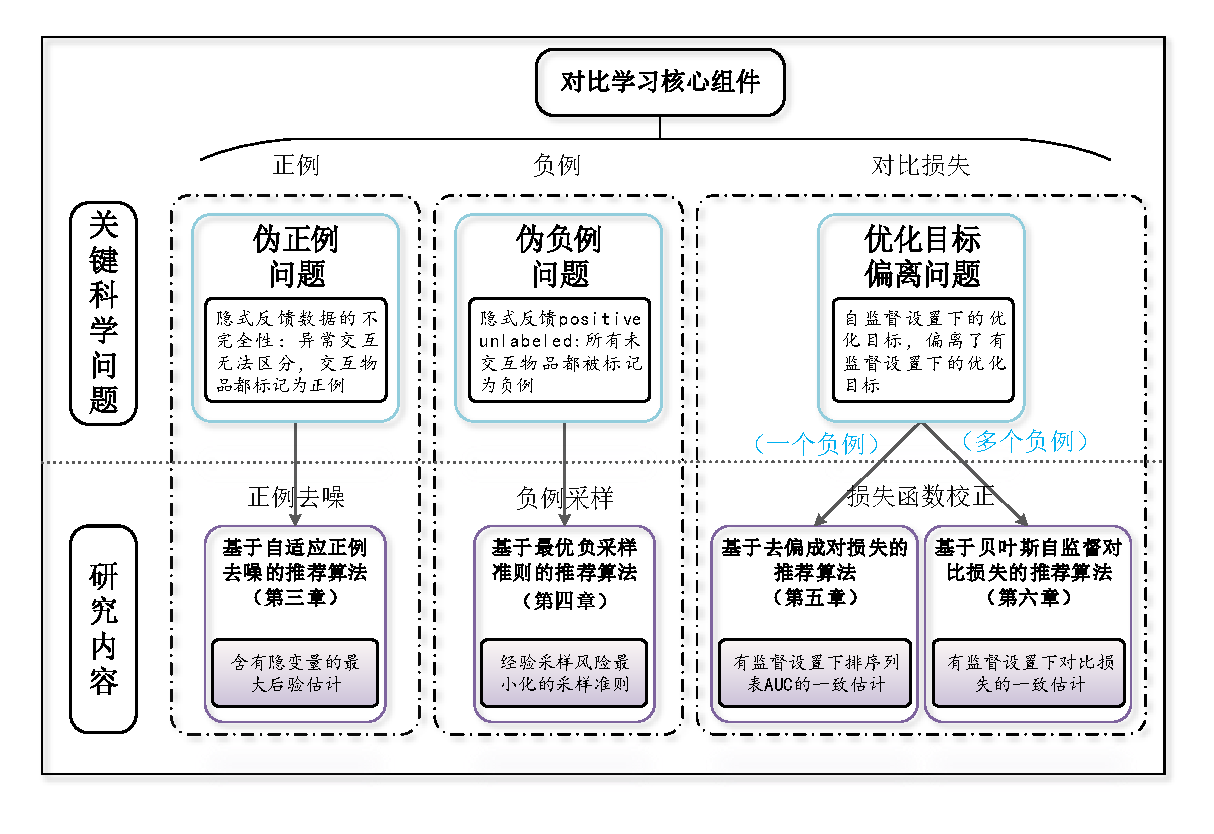
\includegraphics[width=\textwidth]{content.pdf}
	\caption{关键问题与研究内容的关系}
	\label{1Fig:content}
\end{figure*}
%*******************************

\textbf{1)自适应去噪的成对排序推荐算法}


针对伪正例问题,分析了隐式反馈的本质是不完全数据(Incomplete Data),并把从含噪成对比较的数据中学习排序的问题形式化为一个含有隐变量的最大后验估计问题。引入一个隐变量作为衡量交互置信度的新指标,这个隐变量与用户物品的特征表示一起作为模型参数一起端到端地学习。所提出的算法采用期望最大化框架:在期望步骤中使用贝叶斯推断来估计交互的置信度指标;在最大化步骤中固定置信度指标,更新参数学习用户和物品的特征表示。该算法在合成的噪声数据集上表现出了更好的鲁棒性,在真实的数据集上表现出更高的推荐准确性。


\textbf{2)基于最优负采样准则的推荐算法}


针对伪负例问题,提出了最优负采样准则,用于从未标记的数据中采样高质量的负例,以提升对比学习的训练效果并提升推荐精度。提出了后验概率意义上的负信号测度,用于度量未标记样本是真负例的概率。它使用了静态的先验信息和动态的样本信息,较好地综合了现有的两种提取负信号的两种主要范式,并为使用辅助信息建模先验概率的方法提供了灵活的接口。而后提出了最优负采样规则,这是最小化经验采样风险的理论最优的采样准则。该负采样算法在采样误差率和采样样本信息量以及推荐准确性上优于同类方法。


\textbf{3)基于去偏成对损失的推荐算法}


针对自监督设置下成对学习优化目标偏离问题,提出了去偏成对损失,通过校正伪负样本导致的概率估计偏差,从而修正梯度以近似完全监督数据的梯度。去偏成对损失是有监督设置下的成对损失的一致估计,以提升推荐模型的泛化性能。所提出的目标函数不需要额外的辅助信息进行监督,也不需要过多的存储和计算开销。在保持严格的相对于成对学习的线性时间复杂度情况下,基于去偏成对损失的推荐算法取得了更高的推荐准确性。


\textbf{4)基于贝叶斯自监督对比损失的推荐算法}


针对自监督设置下对比学习优化目标偏离问题,提出了贝叶斯自监督对比损失,通过重要性权重来纠正从无标签数据中随机选择的负样本引入的偏差。从单个权重来看,它是未标注样本为真负例的后验概率估计,可以灵活统一地执行硬负例挖掘和伪负例去偏任务这两个矛盾的任务。从损失函数的数值来看,贝叶斯自监督对比损失是有监督设置下的对比损失的一致估计,从而提升推荐模型的泛化性能。只需修改对比损失函数,并且无需额外的存储和计算开销,基于贝叶斯自监督对比损失的推荐算法取得了更高的推荐准确性。此外,在数值实验、图像分类等任务上也验证了贝叶斯自监督对比损失的有效性。

本文共分七章,第一章绪论部分主要介绍了研究背景及意义。第二章介绍了自监督推荐算法和对比学习的基础理论与相关工作。第三、四、五、六章介绍主要研究内容。第七章对全文进行总结,并指出存在的问题及未来可能的发展方向。




